\begin{frame}{Kodierer Information}

\begin{itemize}
\tightlist
\item
  Nicht-Rekursiver Kodierer
\item
  Anzahl von Ausgängen : \[N=2\]
\item
  Anzahl von Registern : \[M=2\]
\item
  Generatoren : \[(1,7)_8 = \begin{pmatrix}001 \\ 111 \\ \end{pmatrix}\]
\end{itemize}

\end{frame}

\begin{frame}{Kodierer Matrix : Nächster Zustand}

\begin{longtable}[c]{@{}lcc@{}}
\toprule
& Bit 0 & Bit 1\tabularnewline
\midrule
\endhead
Zustand 1 & 0 & 2\tabularnewline
Zustand 2 & 2 & 0\tabularnewline
Zustand 3 & 3 & 1\tabularnewline
Zustand 4 & 1 & 3\tabularnewline
\bottomrule
\end{longtable}

\end{frame}

\begin{frame}{Kodierer Matrix : Ausgangsbits}

\begin{longtable}[c]{@{}lcc@{}}
\toprule
& Bit 0 & Bit 1\tabularnewline
\midrule
\endhead
Zustand 1 & 00 & 11\tabularnewline
Zustand 2 & 00 & 11\tabularnewline
Zustand 3 & 01 & 10\tabularnewline
Zustand 4 & 01 & 10\tabularnewline
\bottomrule
\end{longtable}

\end{frame}

\begin{frame}{Kodierer Matrix : Zustandsdiagramm}

\begin{center}
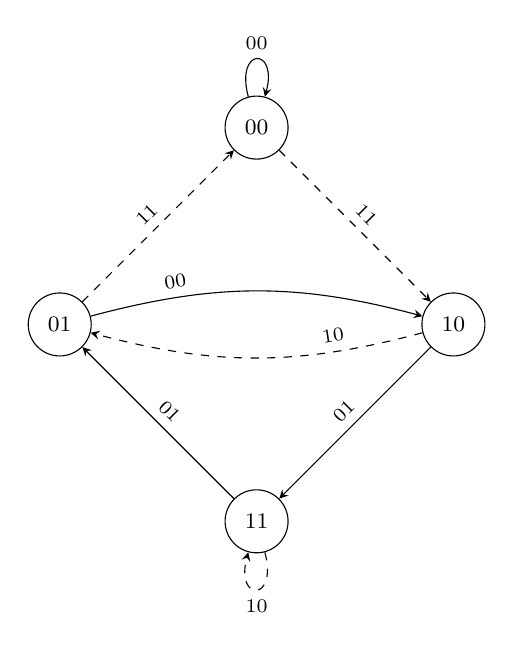
\begin{tikzpicture}[>=stealth, font=\scriptsize]
\tikzstyle{state} = [draw, circle, inner sep=1mm, minimum size=8mm, font=\footnotesize]

 \node[state] (state0) at (0,2.5) {00}; \node[state] (state2) at (2.5,1.53075794227797e-16) {10}; \node[state] (state3) at (3.06151588455594e-16,-2.5) {11}; \node[state] (state1) at (-2.5,-4.59227382683391e-16) {01}; \draw[->] (state0) to [looseness=8,out=105,in=75] node [sloped, above] {00} (state0) ; \draw[->, dashed] (state0) to  node [sloped, above] {11} (state2) ; \draw[->] (state1) to [bend left=15] node [sloped, above,near start] {00} (state2) ; \draw[->, dashed] (state1) to  node [sloped, above] {11} (state0) ; \draw[->] (state2) to  node [sloped, above] {01} (state3) ; \draw[->, dashed] (state2) to [bend left=15] node [sloped, above,near start] {10} (state1) ; \draw[->] (state3) to  node [sloped, above] {01} (state1) ; \draw[->, dashed] (state3) to [looseness=8,out=285,in=255] node [sloped, below] {10} (state3) ;

\end{tikzpicture}
\end{center}

\end{frame}

\begin{frame}{Turbo-Kodierer Information}

\begin{itemize}
\tightlist
\item
  Interleaver : (1, 2, 3, 4, 5, 6, 7)
\item
  Kode-Rate : \[\frac{1}{3}\]
\end{itemize}

\end{frame}

\begin{frame}{Turbo-Kodierer}

\begin{itemize}
\tightlist
\item
  Input : 1, 1, 1, 0, 0, 0, 1, 1, 1, 1, 1, 1, 1, 1, 1, 1, 1, 1, 1, 1,
  \ldots{}
\end{itemize}

\begin{center}
\begin{tikzpicture}[node distance=8mm, inner sep=2mm, outer sep=0, >=stealth, font=\tiny]

\tikzstyle{encoderStyle} = [rectangle, draw, minimum height=height("Inp")+4mm]
\tikzstyle{interleaverStyle} = [encoderStyle]
\tikzstyle{startEndStyle} = [encoderStyle]
\tikzstyle{multiplexerStyle} = [encoderStyle]
\tikzstyle{showStyle} = [rectangle, draw, thick, draw=red, text=red, inner sep=1.5mm]
\tikzstyle{arrowStyle} = [->]
\tikzstyle{showDrawStyle} = [->, red, thick]

\node [interleaverStyle] (interleaver) {Interleaver};
\node [encoderStyle] (encoder1) [above right=of interleaver] {Kodierer 1};
\node [encoderStyle] (encoder2) [below right=of interleaver] {Kodierer 2};
\node [] (multiplexerTemp) [right=of encoder1] {};
\node [multiplexerStyle, rotate=90] (multiplexer) at (multiplexerTemp.east) {Multiplexer};
\node [startEndStyle] (start) [above left=of interleaver] {Input};
\node [startEndStyle] (end) [right=of multiplexerTemp] {Output};

\draw [arrowStyle] (interleaver.south) |- node (afterInterleaver) {}(encoder2.west);
\draw [arrowStyle] (encoder1.east) -- node (afterParity1) {} (multiplexer.north);
\draw [arrowStyle] (start.east)  -| node[midway] (afterInput) {} (interleaver.north);
\draw [arrowStyle] (afterInput.center) |- (encoder1.west);
\draw [arrowStyle] (encoder2.east) -| ++(0.2,0.7) node (afterParity2) {} |- ($(multiplexer.north)+(0,-.5)$);
\draw [arrowStyle] (afterInput.center) |- ($(multiplexer.north)+(0,.5)$);
\draw [arrowStyle] (multiplexer.south) -- node (afterMultiplexer) {} (end.west);

\begin{scope}[on background layer]
\node [draw, fit=(encoder1) (interleaver) (encoder2) (multiplexer)] (background) {};
\end{scope}

\visible<2>{
  \node [showStyle] (showAbove) [above=4mm of background] {\textbf{1, 1, 1, 0, 0, 0, 1, 1, 1, 1, 1, 1, 1, 1, 1, 1, 1, 1, 1, 1, ...}};
  \draw [showDrawStyle] (showAbove) -- (afterInput.center);
  \node [showStyle] (showBelow) [below=4mm of background] {\textbf{3, 1, 1, 0, 0, 0, 1, 1, 1, 1, 1, 1, 1, 1, 1, 1, 1, 1, 1, 1, ...}};
  \draw [showDrawStyle] (showBelow) -- (afterParity1.center);
  }
\visible<3>{
  \node [showStyle] (showAbove) [above=4mm of background] {\textbf{1, 1, 1, 0, 0, 0, 1, 1, 1, 1, 1, 1, 1, 1, 1, 1, 1, 1, 1, 1, ...}};
  \draw [showDrawStyle] (showAbove) -- (afterInput.center);
  \node [showStyle] (showBelow) [below=4mm of background] {\textbf{2, 1, 1, 0, 0, 0, 1, 1, 1, 1, 1, 1, 1, 1, 1, 1, 1, 1, 1, 1, ...}};
  \draw [showDrawStyle] (showBelow) -- (afterInterleaver.center);
  }
\visible<4>{
  \node [showStyle] (showAbove) [above=4mm of background] {\textbf{4, 1, 1, 0, 0, 0, 1, 1, 1, 1, 1, 1, 1, 1, 1, 1, 1, 1, 1, 1, ...}};
  \draw [showDrawStyle] (showAbove) -- (afterParity2.center);
  \node [showStyle] (showBelow) [below=4mm of background] {\textbf{2, 1, 1, 0, 0, 0, 1, 1, 1, 1, 1, 1, 1, 1, 1, 1, 1, 1, 1, 1, ...}};
  \draw [showDrawStyle] (showBelow) -- (afterInterleaver.center);
  }

\end{tikzpicture}
\end{center}

\begin{itemize}
\tightlist
\item
  Output : 5, 1, 1, 0, 0, 0, 1, 1, 1, 1, 1, 1, 1, 1, 1, 1, 1, 1, 1, 1,
  1, 1, 1, 0, 0, 0, 1, 1, 1, 1, 1, 1, 1, 1, 1, 1, 1, 1, 1, 1, 1, 1, 1,
  0, 0, \ldots{}
\end{itemize}

\end{frame}
